\section{Driving Smoothness}
\label{sec:Results_Smoothness}

The analysis of driving smoothness examines the average acceleration, $\gls{a}$, and average jerk, $\gls{j}$, as functions of the \ac{mpr}. Table~\vref{tab:DrivingSmoothness} reports the paired values $(\gls{a}, \gls{j})$ for the Standard, \ac{flow-glosa}, and \ac{eco-glosa} configurations under both emission models. Figures~\vref{fig:Smoothness_692}, \vref{fig:Smoothness_2769}, and \vref{fig:Smoothness_3462} illustrate these trends at representative traffic volumes.

\paragraph{Low to Intermediate Demand ($69$--$692~\unit{\veh\per\hour}$).}
In this regime, \ac{eco-glosa} consistently establishes an inverse relationship between average acceleration and jerk as \ac{mpr} increases. At a demand of $69~\unit{\veh\per\hour}$ with the HBEFA4 model, acceleration falls from $0.30~\unit{\metre\per\second\squared}$ to $0.25~\unit{\metre\per\second\squared}$ (a $17\%$ reduction), while jerk rises from $0.74~\unit{\metre\per\second\cubed}$ to $0.81~\unit{\metre\per\second\cubed}$ (a $9\%$ increase). This pattern, where gentler accelerations are offset by sharper adjustments, is illustrated in Figure~\vref{fig:Smoothness_692}. In comparison, the \ac{flow-glosa} controller offers more balanced improvements, reducing average acceleration by approximately $15\%$ to $20\%$ from the Standard with only a minimal corresponding increase in average jerk, thereby maintaining a more stable overall profile.

\begin{figure}[htbp]
  \centering
  \begin{subfigure}[b]{0.98\textwidth}
    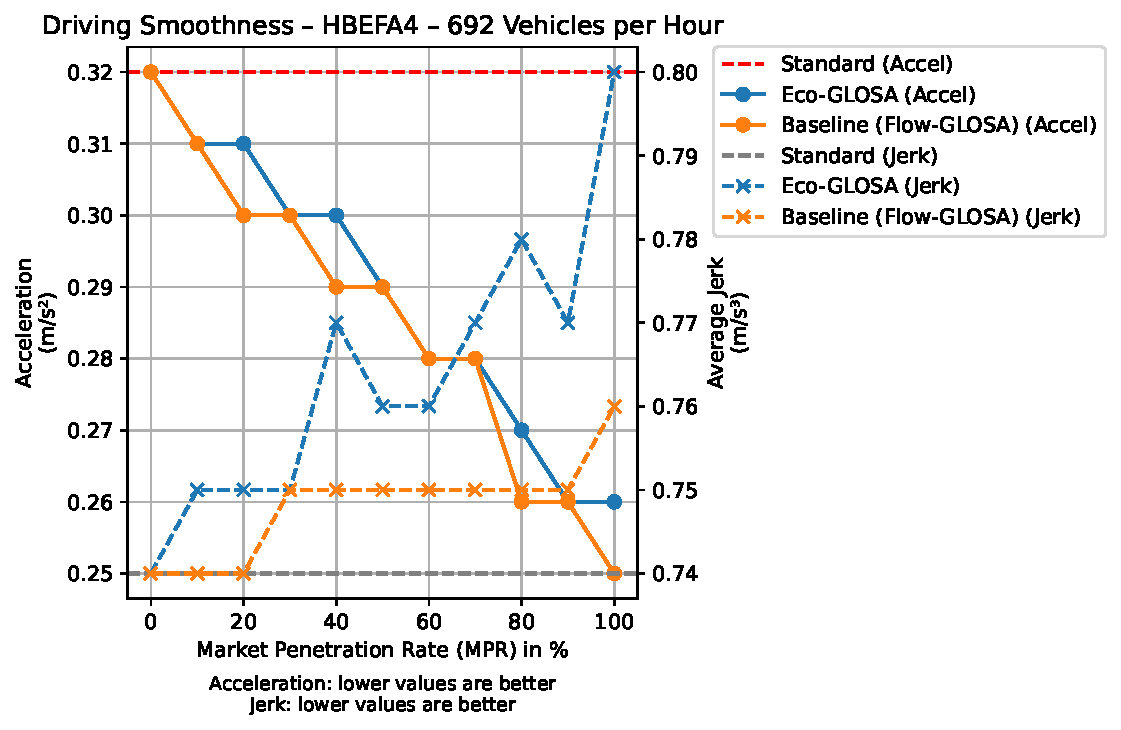
\includegraphics[width=\textwidth]{data/img/DrivingSmoothness/DrivingSmoothness_HBEFA4_Cars692.pdf}
    \caption{Results under the HBEFA4 emission model.}
    \label{fig:Smoothness_HBEFA4_692}
  \end{subfigure}
  \begin{subfigure}[b]{0.98\textwidth}
    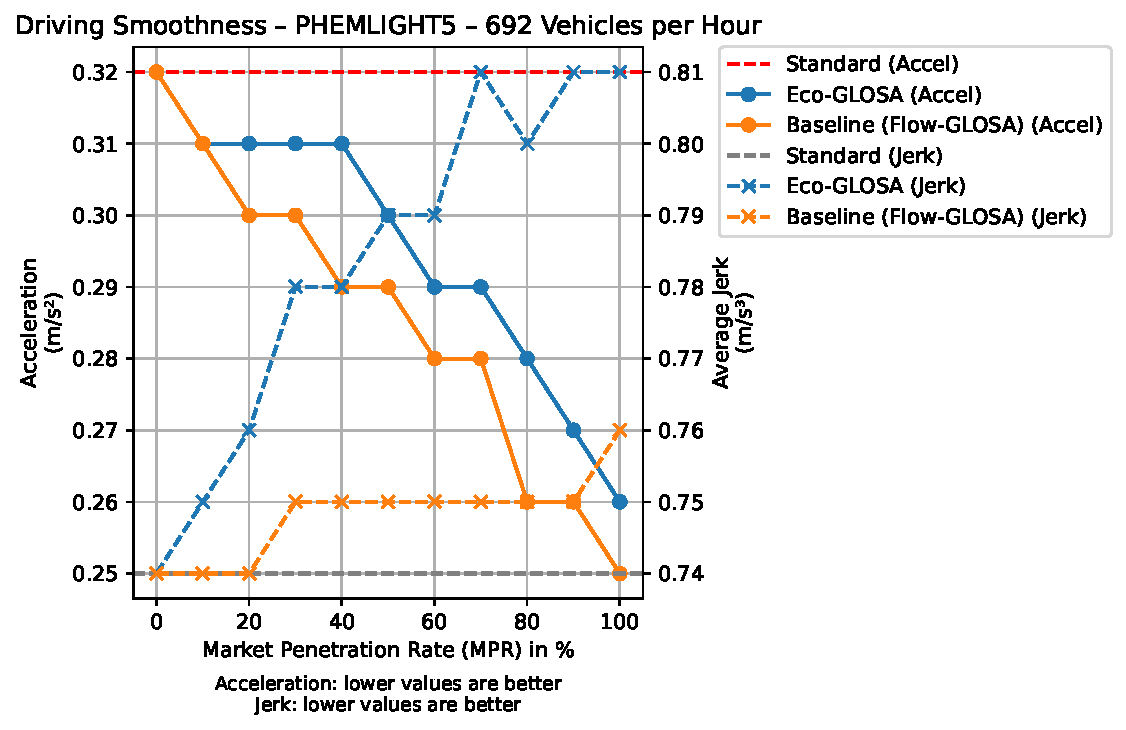
\includegraphics[width=\textwidth]{data/img/DrivingSmoothness/DrivingSmoothness_PHEMLIGHT5_Cars692.pdf}
    \caption{Results under the PHEMlight5 emission model.}
    \label{fig:Smoothness_PHEMlight5_692}
  \end{subfigure}
  \caption[Driving smoothness metrics at $692~\unit{\veh\per\hour}$]{Driving smoothness metrics at a moderate demand of $692~\unit{\veh\per\hour}$. The plots compare average acceleration and jerk for the Standard, \ac{eco-glosa}, and \ac{flow-glosa} controllers.}
  \label{fig:Smoothness_692}
\end{figure}

\paragraph{Emerging Congestion ($1385$--$2077~\unit{\veh\per\hour}$).}
As demand approaches the network's capacity, the trends established at lower volumes continue. Under \ac{eco-glosa}, the trade-off between decreasing acceleration and increasing jerk persists. For the \ac{flow-glosa} controller, both smoothness metrics remain stable and generally improve upon the Standard scenario. At $2077~\unit{\veh\per\hour}$, for instance, \ac{flow-glosa} reduces the baseline acceleration of $0.34~\unit{\metre\per\second\squared}$ down to $0.26~\unit{\metre\per\second\squared}$ at full penetration, while keeping jerk levels steady. This indicates its ability to maintain smooth traffic flow even as the system becomes emphasized.

\paragraph{High Demand ($2769~\unit{\veh\per\hour}$).}
At the jam threshold, driving smoothness under \ac{eco-glosa} becomes highly dependent on the emission model (Figure~\vref{fig:Smoothness_2769}). The HBEFA4 model shows fluctuating acceleration values, whereas the PHEMlight5 model achieves a more favourable outcome. This divergence occurs because vehicles under the PHEMlight5 model adopt more conservative, slower speeds to minimise acceleration events, as established in the previous sections. This inherently cautious behaviour prevents the wide fluctuations observed with the HBEFA4 model. Consequently, jerk declines to $0.66~\unit{\metre\per\second\cubed}$, a value $13\%$ below the Standard of $0.76~\unit{\metre\per\second\cubed}$. This suggests that once vehicles navigate the initial stop-and-go waves, their subsequent trajectories are smoother. Throughout this volatile regime, \ac{flow-glosa} continues to provide stable and predictable smoothness benefits.

\begin{figure}[htbp]
  \centering
  \begin{subfigure}[b]{0.98\textwidth}
    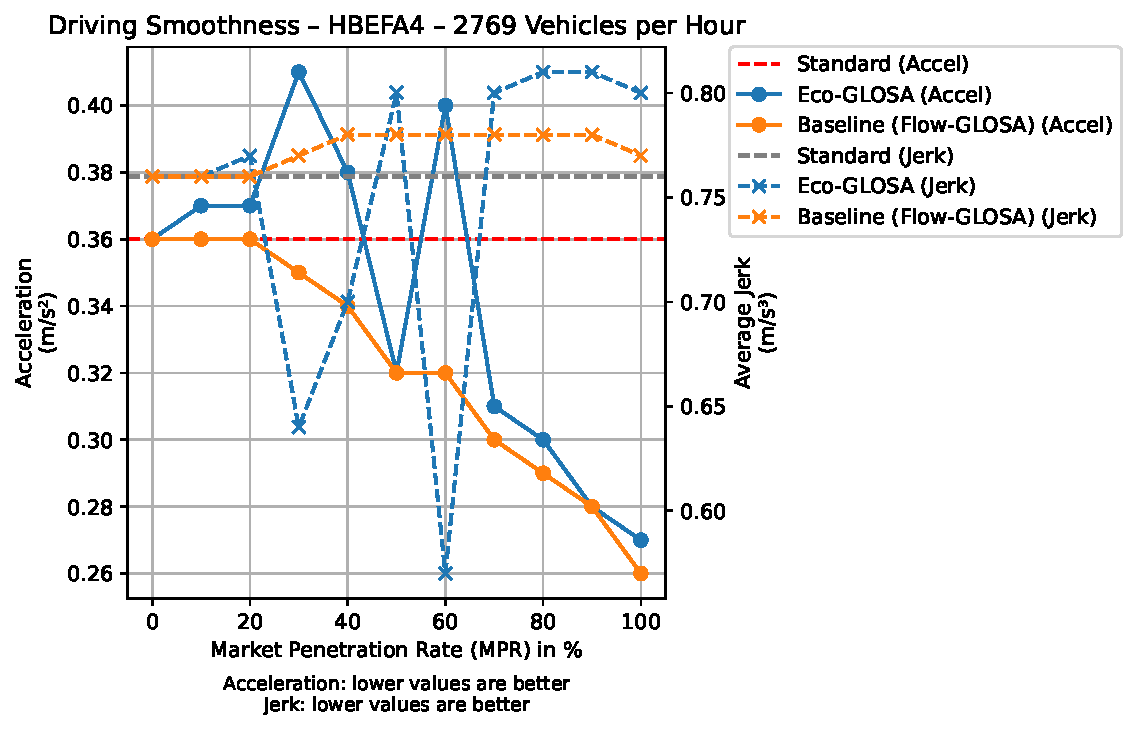
\includegraphics[width=\textwidth]{data/img/DrivingSmoothness/DrivingSmoothness_HBEFA4_Cars2769.pdf}
    \caption{Performance with the HBEFA4 emission model.}
    \label{fig:Smoothness_HBEFA4_2769}
  \end{subfigure}
  \begin{subfigure}[b]{0.98\textwidth}
    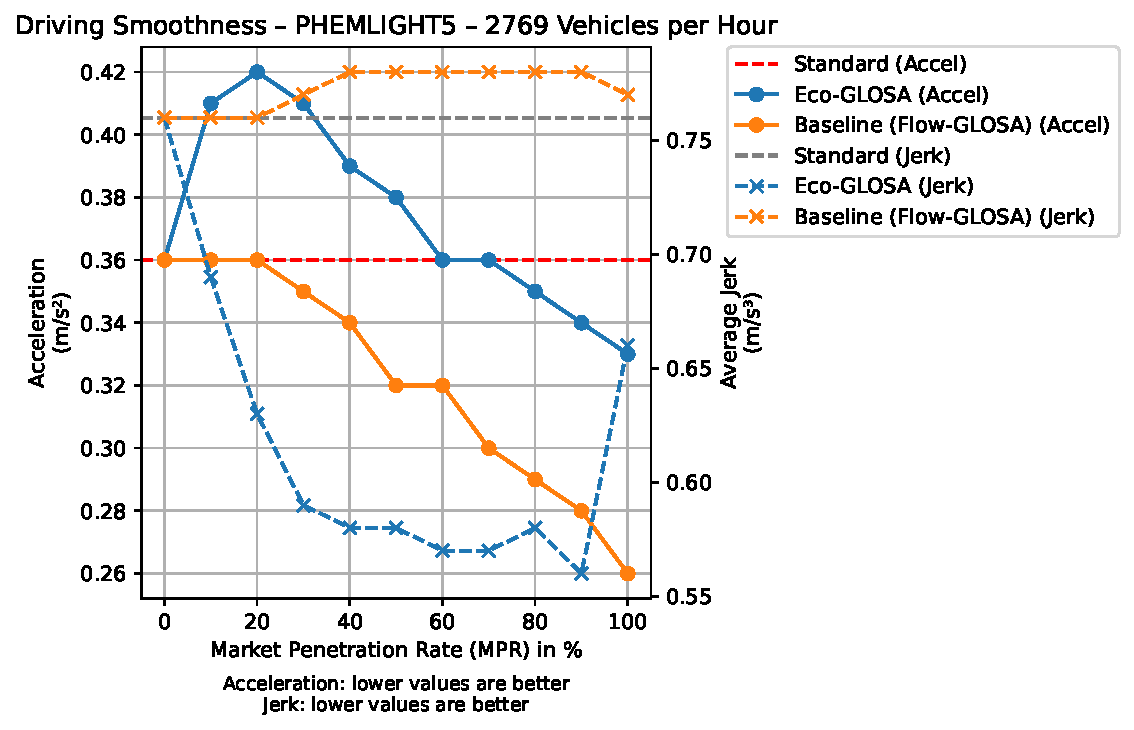
\includegraphics[width=\textwidth]{data/img/DrivingSmoothness/DrivingSmoothness_PHEMLIGHT5_Cars2769.pdf}
    \caption{Performance with the PHEMlight5 emission model.}
    \label{fig:Smoothness_PHEMlight5_2769}
  \end{subfigure}
  \caption[Driving smoothness vs. \ac{mpr} at $2769~\unit{\veh\per\hour}$]{Driving smoothness as a function of \ac{mpr} at the jam threshold of $2769~\unit{\veh\per\hour}$. The plots show the performance of the three controller strategies under two emission models.}
  \label{fig:Smoothness_2769}
\end{figure}

\paragraph{Saturated Regime ($3462~\unit{\veh\per\hour}$).}
In the fully saturated regime, where the system is already gridlocked, \ac{eco-glosa} yields clear improvements in both smoothness metrics as \ac{mpr} increases. For HBEFA4, acceleration decreases from $0.55$ to $0.38~\unit{\metre\per\second\squared}$ and jerk from $0.57$ to $0.51~\unit{\metre\per\second\cubed}$. However, this must be interpreted within the context of a persistent traffic jam. The data does not indicate a dissolution of the queue, but rather suggests that the controller successfully modifies the \enquote{character} of the stop-and-go waves from aggressive manoeuvres to a smoother, less frantic \enquote{creeping} behaviour. In contrast, the \ac{flow-glosa} controller's dynamics shift significantly as it prevents gridlock. It exhibits a notable jerk spike from $0.59~\unit{\metre\per\second\cubed}$ to $0.71~\unit{\metre\per\second\cubed}$ at $60\%$ \ac{mpr}. This transient, which is a necessary trade-off for preserving network capacity, precisely corresponds to the point at which traffic waves are absent and cars can travel at free-flowing speeds.

\begin{figure}[htbp]
  \centering
  \begin{subfigure}[b]{0.98\textwidth}
    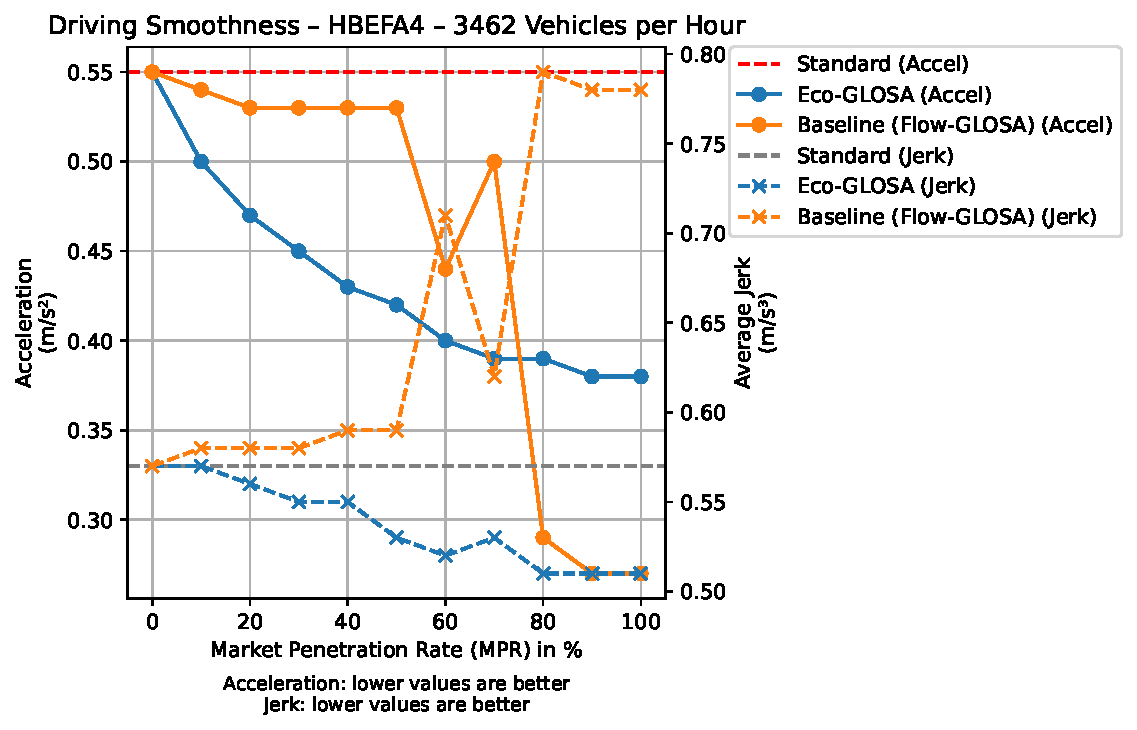
\includegraphics[width=\textwidth]{data/img/DrivingSmoothness/DrivingSmoothness_HBEFA4_Cars3462.pdf}
    \caption{Simulation results using the HBEFA4 model.}
    \label{fig:Smoothness_HBEFA4_3462}
  \end{subfigure}
  \begin{subfigure}[b]{0.98\textwidth}
    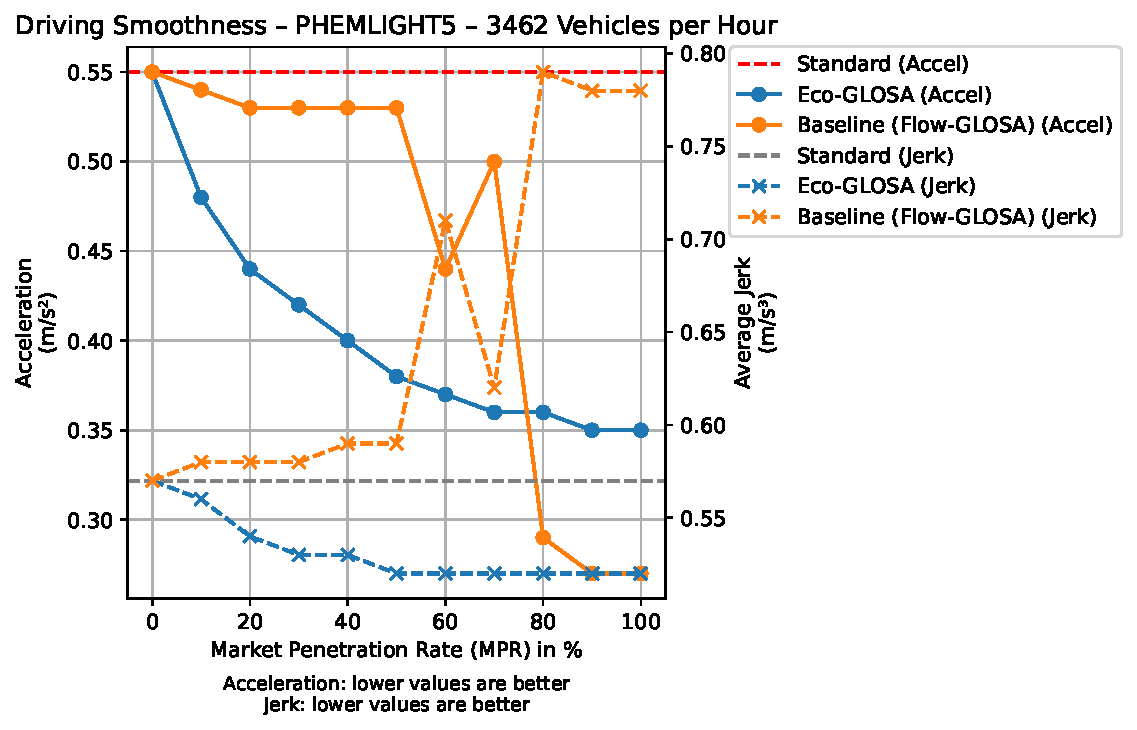
\includegraphics[width=\textwidth]{data/img/DrivingSmoothness/DrivingSmoothness_PHEMLIGHT5_Cars3462.pdf}
    \caption{Simulation results using the PHEMlight5 model.}
    \label{fig:Smoothness_PHEMlight5_3462}
  \end{subfigure}
  \caption[Driving smoothness metrics at $3462~\unit{\veh\per\hour}$]{Driving smoothness metrics in the fully saturated regime ($3462~\unit{\veh\per\hour}$). The plots compare the Standard, \ac{eco-glosa}, and \ac{flow-glosa} controllers.}
  \label{fig:Smoothness_3462}
\end{figure}

\paragraph{Implications.}
The analysis reveals two distinct approaches to driving smoothness. The \ac{eco-glosa} controller consistently attempts to smooth trajectories regardless of the traffic state. In unsaturated conditions, this results in a trade-off where lower average accelerations are achieved at the cost of higher jerk. In saturated conditions, this same logic improves ride comfort by changing the nature of the traffic jam to a smoother progressive motion, but it fails to address the underlying congestion. The \ac{flow-glosa} controller, prioritising throughput, provides balanced smoothness improvements in unsaturated states and accepts a temporary spike in jerk as a necessary by-product of successfully preventing network collapse under saturated conditions. It is important to contextualise these smoothness metrics, however. The high jerk values observed --- both those from the frequent micro-adjustments in the \ac{eco-glosa} strategy and the transient spike from \ac{flow-glosa} --- are likely artifacts of the simulation. In real-world high-demand or congested conditions, human drivers would not replicate such rapid, small-scale accelerations, meaning these specific values are primarily relevant for comparing controller behaviour within the simulation environment rather than predicting on-road performance.

\paragraph{Key Takeaways.}
\begin{enumerate}
    \item \textbf{Unsaturated Conditions:} In low to intermediate demand, \ac{eco-glosa} reduces average acceleration at the cost of higher average jerk. \ac{flow-glosa} provides a more balanced improvement, reducing acceleration while keeping jerk stable.
    \item \textbf{Saturated \ac{eco-glosa} Performance:} In fully saturated, gridlocked conditions, \ac{eco-glosa} significantly improves driving smoothness. It does not prevent the traffic jam but transforms its dynamics from rapidly moving stop-and-go waves into a more comfortable, low-acceleration progressive flow.
    \item \textbf{Saturated \ac{flow-glosa} Performance:} The \ac{flow-glosa} controller's primary objective is to prevent gridlock. This can result in a transient spike in jerk, which signifies the successful absorption of traffic waves as the system transitions from a near-congested to a free-flow state.
    \item \textbf{Controller Philosophy Trade-off:} The results highlight a fundamental trade-off. \ac{eco-glosa} optimises for smooth driving within a given traffic state, even if that state is congested. \ac{flow-glosa} optimises to maintain a smooth, uncongested state, accepting momentary lapses in smoothness to achieve this goal.
\end{enumerate}

\begin{table}[htb]
  \centering
  \caption[Average acceleration and jerk across all volumes and \acp{mpr}]{Driving smoothness, detailed by average acceleration ($\unit{\metre\per\second\squared}$) and jerk ($\unit{\metre\per\second\cubed}$), across all traffic volumes and \acp{mpr}. Results are provided for the Standard, \ac{flow-glosa}, and \ac{eco-glosa} configurations.}
  \label{tab:DrivingSmoothness}
  \resizebox{\textwidth}{!}{%
    \begin{tabular}{l l l *{11}{c}}
      \toprule
      Vehicles & Algorithm & Model       & \textbf{0\% (Standard)} & 10\%        & 20\%        & 30\%        & 40\%        & 50\%        & 60\%        & 70\%        & 80\%        & 90\%        & 100\%       \\
      \midrule
      \textbf{69.0}  & Eco-GLOSA                   & HBEFA4      & \textbf{0.3, 0.74}   & 0.29, 0.75  & 0.31, 0.76  & 0.28, 0.77  & 0.29, 0.77  & 0.29, 0.79  & 0.27, 0.77  & 0.25, 0.81  & 0.28, 0.80  & 0.24, 0.79  & 0.25, 0.81  \\
      \textbf{69.0}  & Baseline (Flow-GLOSA)       & HBEFA4      & \textbf{0.3, 0.74}   & 0.29, 0.76  & 0.31, 0.75  & 0.28, 0.75  & 0.28, 0.75  & 0.29, 0.75  & 0.28, 0.74  & 0.25, 0.75  & 0.27, 0.75  & 0.25, 0.75  & 0.25, 0.77  \\
      \textbf{69.0}  & Eco-GLOSA                   & PHEMlight5  & \textbf{0.3, 0.74}   & 0.29, 0.76  & 0.29, 0.75  & 0.28, 0.76  & 0.27, 0.78  & 0.28, 0.78  & 0.27, 0.80  & 0.25, 0.81  & 0.27, 0.80  & 0.24, 0.79  & 0.23, 0.81  \\
      \textbf{69.0}  & Baseline (Flow-GLOSA)       & PHEMlight5  & \textbf{0.3, 0.74}   & 0.29, 0.76  & 0.31, 0.75  & 0.28, 0.75  & 0.28, 0.75  & 0.29, 0.75  & 0.28, 0.74  & 0.25, 0.75  & 0.27, 0.75  & 0.25, 0.75  & 0.25, 0.77  \\
      \midrule
      \textbf{138.0} & Eco-GLOSA                   & HBEFA4      & \textbf{0.31, 0.73}  & 0.29, 0.74  & 0.30, 0.74  & 0.28, 0.74  & 0.28, 0.77  & 0.27, 0.76  & 0.28, 0.77  & 0.25, 0.77  & 0.27, 0.78  & 0.26, 0.79  & 0.25, 0.78  \\
      \textbf{138.0} & Baseline (Flow-GLOSA)       & HBEFA4      & \textbf{0.31, 0.73}  & 0.29, 0.74  & 0.30, 0.75  & 0.30, 0.73  & 0.28, 0.75  & 0.28, 0.74  & 0.27, 0.75  & 0.26, 0.74  & 0.27, 0.75  & 0.26, 0.74  & 0.25, 0.75  \\
      \textbf{138.0} & Eco-GLOSA                   & PHEMlight5  & \textbf{0.31, 0.73}  & 0.30, 0.73  & 0.29, 0.75  & 0.28, 0.75  & 0.28, 0.77  & 0.26, 0.76  & 0.26, 0.78  & 0.26, 0.77  & 0.26, 0.79  & 0.25, 0.79  & 0.24, 0.79  \\
      \textbf{138.0} & Baseline (Flow-GLOSA)       & PHEMlight5  & \textbf{0.31, 0.73}  & 0.29, 0.74  & 0.30, 0.75  & 0.30, 0.73  & 0.28, 0.75  & 0.28, 0.74  & 0.27, 0.75  & 0.26, 0.74  & 0.27, 0.75  & 0.26, 0.74  & 0.25, 0.75  \\
      \midrule
      \textbf{346.0} & Eco-GLOSA                   & HBEFA4      & \textbf{0.31, 0.74}  & 0.31, 0.75  & 0.31, 0.76  & 0.30, 0.76  & 0.29, 0.76  & 0.29, 0.77  & 0.28, 0.77  & 0.28, 0.77  & 0.27, 0.77  & 0.26, 0.79  & 0.25, 0.80  \\
      \textbf{346.0} & Baseline (Flow-GLOSA)       & HBEFA4      & \textbf{0.31, 0.74}  & 0.31, 0.76  & 0.30, 0.75  & 0.30, 0.76  & 0.29, 0.76  & 0.29, 0.76  & 0.27, 0.75  & 0.28, 0.75  & 0.26, 0.76  & 0.26, 0.76  & 0.24, 0.76  \\
      \textbf{346.0} & Eco-GLOSA                   & PHEMlight5  & \textbf{0.31, 0.74}  & 0.31, 0.75  & 0.31, 0.77  & 0.30, 0.77  & 0.29, 0.77  & 0.28, 0.80  & 0.28, 0.79  & 0.28, 0.78  & 0.26, 0.79  & 0.26, 0.80  & 0.25, 0.82  \\
      \textbf{346.0} & Baseline (Flow-GLOSA)       & PHEMlight5  & \textbf{0.31, 0.74}  & 0.31, 0.76  & 0.30, 0.75  & 0.30, 0.76  & 0.29, 0.76  & 0.29, 0.76  & 0.27, 0.75  & 0.28, 0.75  & 0.26, 0.76  & 0.26, 0.76  & 0.24, 0.76  \\
      \midrule
      \textbf{692.0} & Eco-GLOSA                   & HBEFA4      & \textbf{0.32, 0.74}  & 0.31, 0.75  & 0.31, 0.75  & 0.30, 0.75  & 0.30, 0.77  & 0.29, 0.76  & 0.28, 0.76  & 0.28, 0.77  & 0.27, 0.78  & 0.26, 0.77  & 0.26, 0.80  \\
      \textbf{692.0} & Baseline (Flow-GLOSA)       & HBEFA4      & \textbf{0.32, 0.74}  & 0.31, 0.74  & 0.30, 0.74  & 0.30, 0.75  & 0.29, 0.75  & 0.29, 0.75  & 0.28, 0.75  & 0.28, 0.75  & 0.26, 0.75  & 0.26, 0.75  & 0.25, 0.76  \\
      \textbf{692.0} & Eco-GLOSA                   & PHEMlight5  & \textbf{0.32, 0.74}  & 0.31, 0.75  & 0.31, 0.76  & 0.31, 0.78  & 0.31, 0.78  & 0.30, 0.79  & 0.29, 0.79  & 0.29, 0.81  & 0.28, 0.80  & 0.27, 0.81  & 0.26, 0.81  \\
      \textbf{692.0} & Baseline (Flow-GLOSA)       & PHEMlight5  & \textbf{0.32, 0.74}  & 0.31, 0.74  & 0.30, 0.74  & 0.30, 0.75  & 0.29, 0.75  & 0.29, 0.75  & 0.28, 0.75  & 0.28, 0.75  & 0.26, 0.75  & 0.26, 0.75  & 0.25, 0.76  \\
      \midrule
      \textbf{1385.0}& Eco-GLOSA                   & HBEFA4      & \textbf{0.33, 0.74}  & 0.33, 0.75  & 0.33, 0.76  & 0.32, 0.77  & 0.31, 0.77  & 0.31, 0.77  & 0.30, 0.78  & 0.29, 0.78  & 0.28, 0.78  & 0.27, 0.78  & 0.26, 0.78  \\
      \textbf{1385.0}& Baseline (Flow-GLOSA)       & HBEFA4      & \textbf{0.33, 0.74}  & 0.33, 0.75  & 0.33, 0.75  & 0.32, 0.76  & 0.31, 0.76  & 0.30, 0.76  & 0.29, 0.76  & 0.29, 0.76  & 0.27, 0.76  & 0.27, 0.76  & 0.26, 0.75  \\
      \textbf{1385.0}& Eco-GLOSA                   & PHEMlight5  & \textbf{0.33, 0.74}  & 0.34, 0.77  & 0.34, 0.79  & 0.34, 0.80  & 0.33, 0.81  & 0.32, 0.82  & 0.32, 0.84  & 0.30, 0.83  & 0.29, 0.83  & 0.28, 0.84  & 0.27, 0.83  \\
      \textbf{1385.0}& Baseline (Flow-GLOSA)       & PHEMlight5  & \textbf{0.33, 0.74}  & 0.33, 0.75  & 0.33, 0.75  & 0.32, 0.76  & 0.31, 0.76  & 0.30, 0.76  & 0.29, 0.76  & 0.29, 0.76  & 0.27, 0.76  & 0.27, 0.76  & 0.26, 0.75  \\
      \midrule
      \textbf{2077.0}& Eco-GLOSA                   & HBEFA4      & \textbf{0.34, 0.75}  & 0.34, 0.75  & 0.35, 0.76  & 0.34, 0.77  & 0.33, 0.78  & 0.32, 0.78  & 0.31, 0.78  & 0.30, 0.79  & 0.29, 0.79  & 0.28, 0.78  & 0.27, 0.78  \\
      \textbf{2077.0}& Baseline (Flow-GLOSA)       & HBEFA4      & \textbf{0.34, 0.75}  & 0.34, 0.76  & 0.34, 0.76  & 0.33, 0.76  & 0.32, 0.77  & 0.32, 0.77  & 0.30, 0.77  & 0.29, 0.77  & 0.28, 0.76  & 0.26, 0.76  & 0.26, 0.76  \\
      \textbf{2077.0}& Eco-GLOSA                   & PHEMlight5  & \textbf{0.34, 0.75}  & 0.36, 0.78  & 0.35, 0.80  & 0.35, 0.82  & 0.34, 0.84  & 0.32, 0.84  & 0.31, 0.85  & 0.31, 0.87  & 0.29, 0.86  & 0.28, 0.86  & 0.27, 0.87  \\
      \textbf{2077.0}& Baseline (Flow-GLOSA)       & PHEMlight5  & \textbf{0.34, 0.75}  & 0.34, 0.76  & 0.34, 0.76  & 0.33, 0.76  & 0.32, 0.77  & 0.32, 0.77  & 0.30, 0.77  & 0.29, 0.77  & 0.28, 0.76  & 0.26, 0.76  & 0.26, 0.76  \\
      \midrule
      \textbf{2769.0}& Eco-GLOSA                   & HBEFA4      & \textbf{0.36, 0.76}  & 0.37, 0.76  & 0.37, 0.77  & 0.41, 0.64  & 0.38, 0.70  & 0.32, 0.80  & 0.40, 0.57  & 0.31, 0.80  & 0.30, 0.81  & 0.28, 0.81  & 0.27, 0.80  \\
      \textbf{2769.0}& Baseline (Flow-GLOSA)       & HBEFA4      & \textbf{0.36, 0.76}  & 0.36, 0.76  & 0.36, 0.76  & 0.35, 0.77  & 0.34, 0.78  & 0.32, 0.78  & 0.32, 0.78  & 0.30, 0.78  & 0.29, 0.78  & 0.28, 0.78  & 0.26, 0.77  \\
      \textbf{2769.0}& Eco-GLOSA                   & PHEMlight5  & \textbf{0.36, 0.76}  & 0.41, 0.69  & 0.42, 0.63  & 0.41, 0.59  & 0.39, 0.58  & 0.38, 0.58  & 0.36, 0.57  & 0.36, 0.57  & 0.35, 0.58  & 0.34, 0.56  & 0.33, 0.66  \\
      \textbf{2769.0}& Baseline (Flow-GLOSA)       & PHEMlight5  & \textbf{0.36, 0.76}  & 0.36, 0.76  & 0.36, 0.76  & 0.35, 0.77  & 0.34, 0.78  & 0.32, 0.78  & 0.32, 0.78  & 0.30, 0.78  & 0.29, 0.78  & 0.28, 0.78  & 0.26, 0.77  \\
      \midrule
      \textbf{3462.0} & \textbf{Eco-GLOSA} & \textbf{HBEFA4} & \textbf{0.55, 0.57} & \textbf{0.50, 0.57} & \textbf{0.47, 0.56} & \textbf{0.45, 0.55} & \textbf{0.43, 0.55} & \textbf{0.42, 0.53} & \textbf{0.40, 0.52} & \textbf{0.39, 0.53} & \textbf{0.39, 0.51} & \textbf{0.38, 0.51} & \textbf{0.38, 0.51} \\
      \textbf{3462.0}& Baseline (Flow-GLOSA)       & HBEFA4      & \textbf{0.55, 0.57}  & 0.54, 0.58  & 0.53, 0.58  & 0.53, 0.58  & 0.53, 0.59  & 0.53, 0.59  & 0.44, 0.71  & 0.50, 0.62  & \textbf{0.29, 0.79}  & \textbf{0.27, 0.78}  & \textbf{0.27, 0.78}  \\
      \textbf{3462.0} & \textbf{Eco-GLOSA} & \textbf{PHEMlight5} & \textbf{0.55, 0.57} & \textbf{0.48, 0.56} & \textbf{0.44, 0.54} & \textbf{0.42, 0.53} & \textbf{0.40, 0.53} & \textbf{0.38, 0.52} & \textbf{0.37, 0.52} & \textbf{0.36, 0.52} & \textbf{0.36, 0.52} & \textbf{0.35, 0.52} & \textbf{0.35, 0.52} \\
      \textbf{3462.0}& Baseline (Flow-GLOSA)       & PHEMlight5  & \textbf{0.55, 0.57}  & 0.54, 0.58  & 0.53, 0.58  & 0.53, 0.58  & 0.53, 0.59  & 0.53, 0.59  & 0.44, 0.71  & 0.50, 0.62  & \textbf{0.29, 0.79}  & \textbf{0.27, 0.78}  & \textbf{0.27, 0.78}  \\
      \bottomrule
    \end{tabular}%
  }
\end{table}
